\documentclass[tikz,border=10pt]{standalone}
\usetikzlibrary{calc,arrows.meta,perspective,3d}

\begin{document}
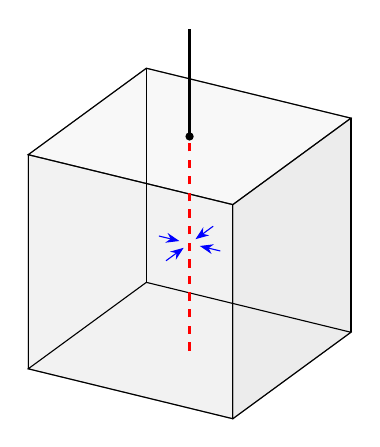
\begin{tikzpicture}[
    >=Stealth,
    3d view={120}{25}, % 3D视角
    scale=1.5
]

% ========== 左侧：3D油藏立方体 ==========
\begin{scope}
    % 定义立方体顶点坐标 (x,y,z)
    \coordinate (O) at (0,0,0);
    \coordinate (A) at (2,0,0);
    \coordinate (B) at (2,2,0);
    \coordinate (C) at (0,2,0);
    \coordinate (O') at (0,0,2);
    \coordinate (A') at (2,0,2);
    \coordinate (B') at (2,2,2);
    \coordinate (C') at (0,2,2);

    % 绘制立方体
    \draw[fill=gray!10, opacity=0.5] (O') -- (A') -- (B') -- (C') -- cycle; % 顶面
    \draw[fill=gray!20, opacity=0.5] (A) -- (A') -- (B') -- (B) -- cycle; % 右侧面
    \draw[fill=gray!30, opacity=0.5] (B) -- (B') -- (C') -- (C) -- cycle; % 前面
    
    % 边框线
    \draw (O) -- (A) -- (B) -- (C) -- cycle; % 底面
    \draw (O') -- (A') -- (B') -- (C') -- cycle; % 顶面
    \draw (A) -- (A') (B) -- (B') (C) -- (C') (O) -- (O'); % 棱边
    \draw[dashed] (O) -- (O'); % 隐藏线

    % 【修正】竖直方向井轨迹（沿z轴）
    \draw[red, line width=1.25pt, dashed] (1,1,0) -- (1,1,2); % 立方体内部竖直段
    \draw[line width=1.25pt] (1,1,2) -- (1,1,3); % 顶部伸出段
    \fill (1,1,2) circle (1pt); % 顶部黑点

    % 【修正】箭头不重叠，分层布置
    % 下层箭头 (z=0.5)
    \draw[blue,->] ($(0.5,1,1)+(0.1,0,0)$) -- ($(1,1,1)-(0.1,0,0)$);
    \draw[blue,->] ($(1.5,1,1)-(0.1,0,0)$) -- ($(1,1,1)+(0.1,0,0)$);
    
    % 中层箭头 (z=1) - 稍长
    \draw[blue,->] ($(1,0.5,1)+(0,0.2,0)$) -- ($(1,1,1)-(0,0.1,0)$);
    \draw[blue,->] ($(1,1.5,1)-(0,0.2,0)$) -- ($(1,1,1)+(0,0.1,0)$);
    
\end{scope}

\end{tikzpicture}
\end{document}